\section{Dataset creation}%TODO:Rewrite without first person !
The original dataset from Wouter\cite{wouter2019} was constructed using \gls{lidar} surveys from a small region of the Netherlands. The data I was given was constructed in the form of a \gls{gis} project, with the position of the different objects being encoded in .shp files. 

A dataset for the training of a Mask-RCNN\cite{maskrcnn} model was also present. It was made from more of a dozen of very high resolution and details tif files, cropped to $600 \times 600$ pixels, and annotated using the COCO\cite{msCOCO} format.

I wanted to create a new dataset that was of a higher resolution, but if each object was annotated and given a position in a given reference system, it was not indicated in which image the object was located. To create a new dataset, I first needed to associate each object with a LiDAR survey image. 

\subsection{Cropping Images}
In order to do this, we first converted the .shp files, which are \gls{gis} specific to CSV using the \href{https://gdal.org/programs/ogr2ogr.html}{\texttt{ogr2ogr}} script. In our case the .shp files contained the position of the bounding boxes of the different objects in the same reference as the image. Each class of objects had its own .shp file. To find out in which image each object where, we needed to also find the coordinates of the images. Luckily, those were encoded in the .tif files themselves. Using \texttt{glalinfo}, we are able to retrieve the position of the image. Finally, we check if all of the vertex of the bounding box of an object are inside of the position of an image to associate it. Using this newly acquired information, we build a new database containing the position of the bounding box, the type of object and in which image this object is in.

\begin{figure}[h!]
  \centering
	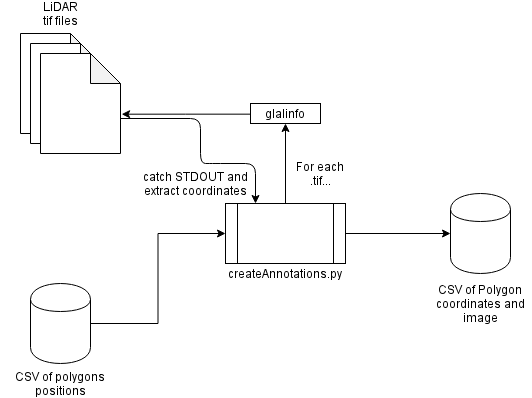
\includegraphics[width=\textwidth]{createAnnotationDiagram}
	\caption[Functionnal Diagram of the createAnnotation script]{Functionnal Diagram of the createAnnotation script. For each objects in the CSV, it cycles for each of the .tif files, extract information concerning its position using the \texttt{glalinfo} program, then if all of the vertex of the bounding box are inside of the image, it adds it to the row of the object, and append it to a new CSV}
  \label{fig:annotationScript}
\end{figure}

We are now in possession of all the necessary information to create a new dataset. This dataset will be created by cropping $1000 \times 1000$ images from the original \gls{lidar} images, which will be centered around an object. This is done for every object in the dataset (around 2K). Luckily, those objects are often cluttered together, meaning that we will often see multiple examples of one class in one image. To create a cropped image, we first need to transform the coordinates of the object, which are from a world reference into a image reference, i.e. between 0 and the length/width of the image. This is done using simple scaling and translating formula, given in Equation \ref{eq:map}. This gives us values that are equivalent to pixels in the image rather than a position in the \gls{gis} world. 

\begin{equation}\label{eq:map}
	f[x] = \frac{x - x_{min}}{x_{max} - x_{min}}*(y_{max} - y_{max}) + y_{min}, 
\end{equation} Where $x_{min}, y_{min}$ are the minimum value of the original range and the destination range respectively, and  where  $x_{min}, y_{min}$ are the maximum value of the original range and the destination range respectively

We center the $1000 \times 1000$ image around those newly transformed values, adding a random jitter value, taken uniformly between $(-100; 100)$. This guarantees us that the image won't be perfectly centered around an object, creating a more difficult image to analyze. Finally, we need to find which objects are in the cropped image. To do so, we iterate through every object in the database, and if they are in the same image, and if all of their vertex are in the cropped section, we add it to the annotation of the image. 

\subsection{Annotations}
Using the scripts, we create a dataset using the already annotated \gls{gis} project. This dataset contains about ~7500 examples, split into a 80/20 train/test dataset. The annotation is done using the COCO format\cite{msCOCO}, where each image is accompanied with a .txt file containing the position of each bounding box, along with its class. The bounding box is position is encoded as  $(x, y, width, height)$, where $x, y$ is the position of the top left corner of the bounding box. Those coordinates are also relative to the image, meaning that $(x,y) \in [0,1] \times [0,1]$. To obtain those bounding box, we again took their position from the .shp file and converted their position from a world reference to a image reference using the same formula as above. We then normalised to obtain values between 0 and 1. 

